\documentclass[xcolor=dvipsnames,table]{beamer} % dvipsnames gives more built-in colors
\usepackage[utf8]{inputenc}
\usepackage[english]{babel}
\usepackage{xcolor}
\usepackage{listings}
\usepackage{caption}
\usepackage{subcaption}
\usepackage{multicol}
\usepackage{xcolor}
\usepackage{pbox}

%%%%%%%%%%%%%%%%%%%%%%%%%%%%%%%%%%%%%%%%%%%%%%%%%%%%%%%%%%%%%%%%%%%%%%%%%%%%%%%%%%%%%%%%%%%%%%%%%%%%%%%%%%%%%%%%%%%%%%%%
%%%%%%%%%%%%%%%%%%%%%%%%%%%%%%%%%%%%%%%%%%%%%% CONFIGURACIONES %%%%%%%%%%%%%%%%%%%%%%%%%%%%%%%%%%%%%%%%%%%%%%%%%%%%%%%%%
%%%%%%%%%%%%%%%%%%%%%%%%%%%%%%%%%%%%%%%%%%%%%%%%%%%%%%%%%%%%%%%%%%%%%%%%%%%%%%%%%%%%%%%%%%%%%%%%%%%%%%%%%%%%%%%%%%%%%%%%

\usetheme{Madrid}
\useoutertheme{miniframes} % Alternatively: miniframes, infolines, split
\useinnertheme{circles}

\definecolor{UBCblue}{rgb}{0.04706, 0.13725, 0.26667} % UBC Blue (primary)
\definecolor{blueapi}{rgb}{0.74, 0.83, 0.9}
\newcommand{\si}{
\includegraphics[height=0.3cm]{../figures/ok-icon.png}}
\newcommand{\no}{
\includegraphics[height=0.3cm]{../figures/x-icon.jpg}}

\lstset{ %
  backgroundcolor=\color{white}, 
  basicstyle=\footnotesize,       
  breakatwhitespace=false,        
  breaklines=true,                 
  captionpos=b,                    
  commentstyle=\color{green},   
  escapeinside={\%*}{*)},        
  extendedchars=true,              
  frame=single,                  
  keywordstyle=\color{blue},       
  language=Prolog,                
  numbers=left,                    
  numbersep=5pt,                   
  numberstyle=\tiny\color{gray},
  rulecolor=\color{black},        
  showspaces=false,               
  showstringspaces=false,          
  showtabs=false,                  
  stepnumber=2,                    
  stringstyle=\color{BrickRed},   
  tabsize=2,                      
  title=\lstname,                  
  morekeywords={not,\},\{,preconditions,effects },            
  deletekeywords={time}            
}

\usecolortheme[named=UBCblue]{structure}
%\usecolortheme[named=Mahogany]{structure} % Sample dvipsnames color

\title[VirtShell]{\textbf{VirtShell} \\ Framework para aprovisionamiento de soluciones virtuales}
\date{\tiny\today}
\titlegraphic{
\includegraphics[width=0.9cm]{logo_univalle.pdf}}
\author[CALlanoR]{\textbf{Carlos Alberto Llano R.}}
\institute[www.univalle.edu.co]{Escuela de Ingeniería de Sistemas y Computación \\ Maestría en Ingeniería con énfasis en Ingeniería de Sistemas y Computación \vspace{0.2cm} \\ Director: \\ \textbf{John Alexander Sanabria}}

\begin{document}

%%%%%%%%%%%%%%%%%%%%%%%%%%%%%%%%%%%%%%%%%%%%%%%%%%%%%%%%%%%%%%%%%%%%%%%%%%%%%%%%%%%%%%%%%%%%%%%%%%%%%%%%%%%%%%%%%%%%%%%%
%%%%%%%%%%%%%%%%%%%%%%%%%%%%%%%%%%%%%%%%%%%%%%%%%%%%% TITULO %%%%%%%%%%%%%%%%%%%%%%%%%%%%%%%%%%%%%%%%%%%%%%%%%%%%%%%%%%%
%%%%%%%%%%%%%%%%%%%%%%%%%%%%%%%%%%%%%%%%%%%%%%%%%%%%%%%%%%%%%%%%%%%%%%%%%%%%%%%%%%%%%%%%%%%%%%%%%%%%%%%%%%%%%%%%%%%%%%%%

\frame{\titlepage}

\setcounter{tocdepth}{1}  % Esto permite esconder las subsections
\frame{\frametitle{Contents}\tableofcontents}

\logo{\hspace*{0.6\textwidth}
\includegraphics[width=0.6cm]{logo_univalle}\hspace*{0.3cm}}

%%%%%%%%%%%%%%%%%%%%%%%%%%%%%%%%%%%%%%%%%%%%%%%%%%%%%%%%%%%%%%%%%%%%%%%%%%%%%%%%%%%%%%%%%%%%%%%%%%%%%%%%%%%%%%%%%%%%%%%%
%%%%%%%%%%%%%%%%%%%%%%%%%%%%%%%%%%%%%%%%%%%%%%%%%%% OBJETIVOS %%%%%%%%%%%%%%%%%%%%%%%%%%%%%%%%%%%%%%%%%%%%%%%%%%%%%%%%%%
%%%%%%%%%%%%%%%%%%%%%%%%%%%%%%%%%%%%%%%%%%%%%%%%%%%%%%%%%%%%%%%%%%%%%%%%%%%%%%%%%%%%%%%%%%%%%%%%%%%%%%%%%%%%%%%%%%%%%%%%

\section{Objetivos}

\frame{ \frametitle{Objetivos}
	\setbeamercolor{block title}{fg=white,bg=blue!75!black}
	\begin{block}{General}
	Diseñar un framework web, que permita el aprovisionamiento de software automático, para ambientes virtualizados.
	\end{block}
	\pause
	\vspace{0.3cm}
	\setbeamercolor{block title}{fg=white,bg=blue!75!black}
	\begin{block}{Específicos}
		\begin{enumerate}
			\item Evaluar diferentes técnicas y soluciones de aprovisionamiento que se utilizan en la actualidad.
			\item Evaluar diferentes mecanismos de aprovisionamiento.
			\item Realizar una ejemplificación del framework.
		\end{enumerate}
	\end{block}
}

%%%%%%%%%%%%%%%%%%%%%%%%%%%%%%%%%%%%%%%%%%%%%%%%%%%%%%%%%%%%%%%%%%%%%%%%%%%%%%%%%%%%%%%%%%%%%%%%%%%%%%%%%%%%%%%%%%%%%%%%
%%%%%%%%%%%%%%%%%%%%%%%%%%%%%%%%%%%%%%%%%%%%%%%%% OBJETIVO #1 %%%%%%%%%%%%%%%%%%%%%%%%%%%%%%%%%%%%%%%%%%%%%%%%%%%%%%%%%%
%%%%%%%%%%%%%%%%%%%%%%%%%%%%%%%%%%%%%%%%%%%%%%%%%%%%%%%%%%%%%%%%%%%%%%%%%%%%%%%%%%%%%%%%%%%%%%%%%%%%%%%%%%%%%%%%%%%%%%%%

\subsection{Técnicas y soluciones de aprovisionamiento actuales (Objetivo \#1)}

\frame{ \frametitle{Técnicas de Virtualización trabajadas}
	\begin{figure}
		\captionsetup[subfigure]{labelformat=empty}
		\begin{subfigure}{.5\textwidth}
			\centering
			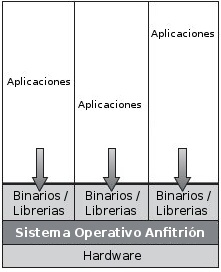
\includegraphics[height=5cm]{../../architecture/v1/diagrams/contenedores.jpg}
			\caption{Contenedores}
		\end{subfigure}%
		\pause
		\begin{subfigure}{.5\textwidth}
			\centering
			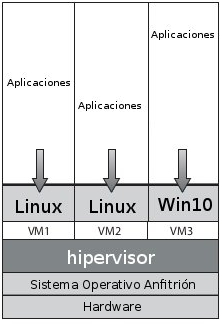
\includegraphics[height=5cm]{../../architecture/v1/diagrams/virtualmachine.jpg}
			\caption{Máquinas Virtuales}
		\end{subfigure}%
	\end{figure}
}

\frame{ \frametitle{Soluciones de aprovisionamiento evaluadas}
\begin{multicols}{2}
	\begin{itemize}
		\item Fabric
		\item Chef
		\item Puppet
		\item Juju
		\item CFEngine
		\item Bcfg2
		\item Ansible
		\item Cobbler
		\item SmartFrog
		\item Amazon EC2
		\item Docker composer
		\item SaltStack
		\item Vagrant
	\end{itemize}
\end{multicols}
}

\frame{ \frametitle{Soluciones de aprovisionamiento evaluadas}
\scriptsize
\begin{tabular}{| l | l | l | l | l | l | l |}
	\hline
	\rowcolor{blueapi}
	\textbf{Solución} & \textbf{Sop.Nubes} & \textbf{Curv.Apren} & \textbf{Crea} & \textbf{Aprov} & \textbf{API REST} & \textbf{Mult.SO} \\ [0.5ex]
	\hline\hline
	Chef          & Todas                           & Alta     & \si     & \si   & \si   & \si   \\ \hline
	Juju          & \pbox{5cm}{OpenStack \\ MAAS}   & Baja     & \si     & \si   & \no   & \no   \\ \hline
	Puppet        & La mayoria                      & Media    & \no     & \si   & \no   & \si   \\ \hline
	Ansible       & \pbox{5cm}{Amazon \\ OpenStack} & Baja     & \no     & \si   & \no   & \si   \\ \hline
	Amazon EC2    & Amazon                          & Media    & \si     & \si   & \si   & \si   \\ \hline
	Docker        & \no                             & Media    & \si     & \si   & \si   & \si   \\ \hline
	Vagrant       & \no                             & Baja     & \si     & \si   & \no   & \si   \\ \hline
\end{tabular}
}

%%%%%%%%%%%%%%%%%%%%%%%%%%%%%%%%%%%%%%%%%%%%%%%%%%%%%%%%%%%%%%%%%%%%%%%%%%%%%%%%%%%%%%%%%%%%%%%%%%%%%%%%%%%%%%%%%%%%%%%%
%%%%%%%%%%%%%%%%%%%%%%%%%%%%%%%%%%%%%%%%%%%%%%%%% OBJETIVO #2 %%%%%%%%%%%%%%%%%%%%%%%%%%%%%%%%%%%%%%%%%%%%%%%%%%%%%%%%%%
%%%%%%%%%%%%%%%%%%%%%%%%%%%%%%%%%%%%%%%%%%%%%%%%%%%%%%%%%%%%%%%%%%%%%%%%%%%%%%%%%%%%%%%%%%%%%%%%%%%%%%%%%%%%%%%%%%%%%%%%

\subsection{Evaluar diferentes mecanismos de aprovisionamiento. (Objetivo \#2)}

\frame{ \frametitle{Estilos de servicios web}
\begin{itemize}
\item RPC
\item REST
\end{itemize}
}

%%%%%%%%%%%%%%%%%%%%%%%%%%%%%%%%%%%%%%%%%%%%%%%%%%%%%%%%%%%%%%%%%%%%%%%%%%%%%%%%%%%%%%%%%%%%%%%%%%%%%%%%%%%%%%%%%%%%%%%%
%%%%%%%%%%%%%%%%%%%%%%%%%%%%%%%%%%%%%%%%%%%%%%%%% OBJETIVO #3 %%%%%%%%%%%%%%%%%%%%%%%%%%%%%%%%%%%%%%%%%%%%%%%%%%%%%%%%%%
%%%%%%%%%%%%%%%%%%%%%%%%%%%%%%%%%%%%%%%%%%%%%%%%%%%%%%%%%%%%%%%%%%%%%%%%%%%%%%%%%%%%%%%%%%%%%%%%%%%%%%%%%%%%%%%%%%%%%%%%

\subsection{Realizar una ejemplificación del framework. (Objetivo \#3)}

\frame{ \frametitle{Framework}
\begin{figure}
	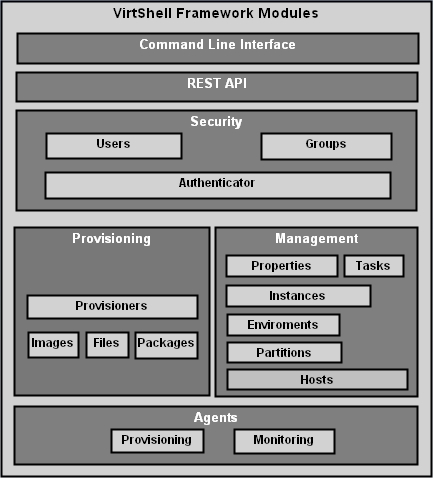
\includegraphics[width = 0.5\textwidth]{../../architecture/v1/diagrams/framework}
\end{figure}
}

\frame{ \frametitle{Flujo de aprovisionamiento}
\begin{figure}
	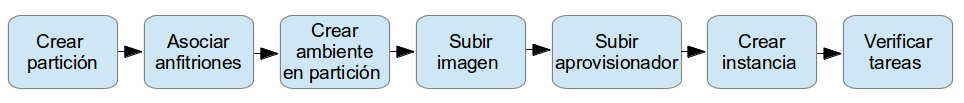
\includegraphics[width = 0.9\textwidth]{../figures/general_workflow_provisioning}
\end{figure}
}

\frame{ \frametitle{Particiones y Anfitriones}
\begin{figure}
	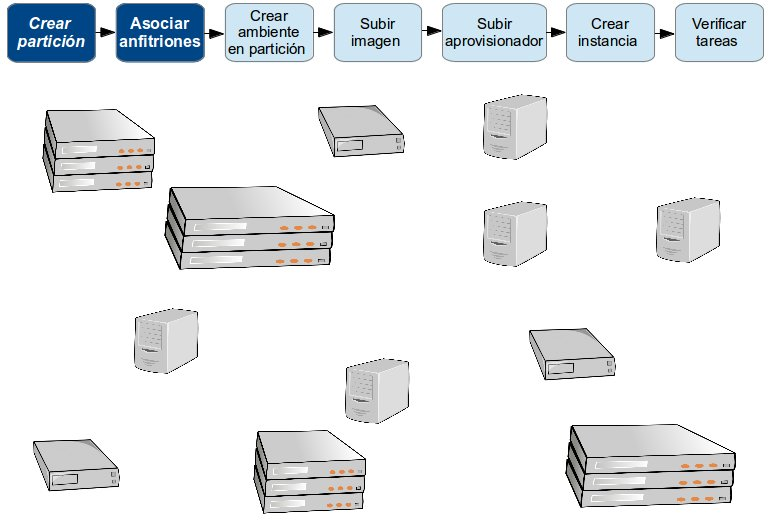
\includegraphics[width = 0.8\textwidth]{../figures/partitions_and_hosts}
\end{figure}
}


\frame{ \frametitle{Particiones y Anfitriones}
\begin{figure}
	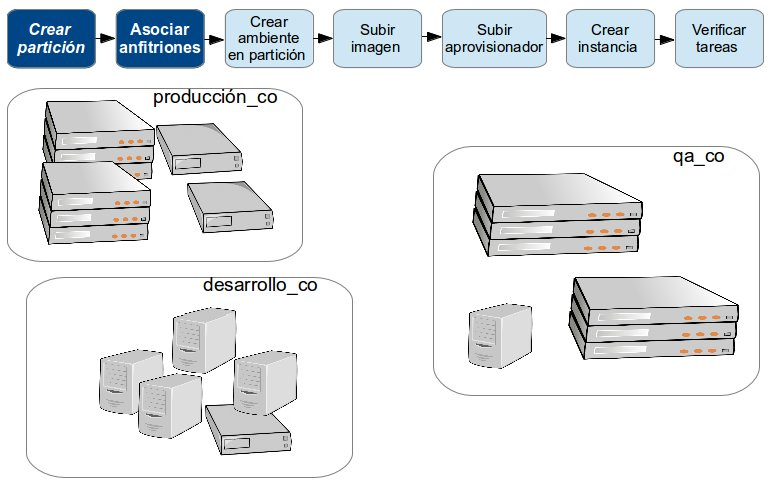
\includegraphics[width = 0.8\textwidth]{../figures/partitions_and_hosts2}
\end{figure}
}

\begin{frame}[fragile]
\frametitle{Particiones y Anfitriones (Ejemplo)}
\begin{lstlisting}[language=Bash,basicstyle=\ttfamily\scriptsize,keywordstyle=\color{blue}]
curl -X POST http://virtshellsrv:80/partitions/ 
    -d "{\"name\":\"development_co\",
         \"description\":\"Collection of servers oriented to development team in Colombia.\"}" 
    -H "accept:application/json" | jq .
\end{lstlisting}
\end{frame}


\frame{ \frametitle{Ambientes de trabajo}
\begin{figure}
	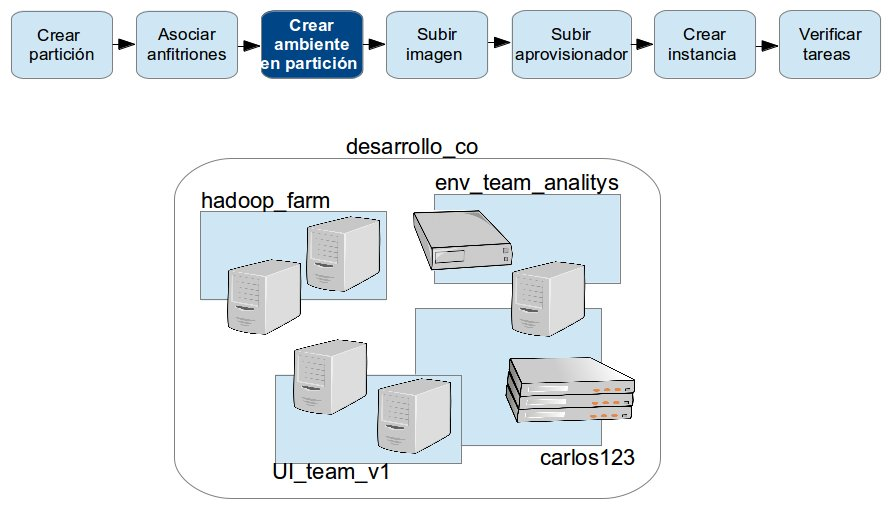
\includegraphics[width = 0.8\textwidth]{../figures/enviroments}
\end{figure}
}

\begin{frame}[fragile]
\frametitle{Ambientes de trabajo (Ejemplo)}
\begin{lstlisting}[language=Bash,basicstyle=\ttfamily\scriptsize,keywordstyle=\color{blue}]
curl -X POST http://virtshellsrv:80/enviroments/ 
    -d "{\"name\":\"development\",
         \"description\":\"Development enviroment\", 
         \"partition\": \"development_co\", 
         \"users\": [{\"login\": \"development_user\"}, 
                     {\"login\": \"guest\"}]}" 
    -H "accept:application/json" | jq .
\end{lstlisting}
\end{frame}

\frame{ \frametitle{Imagenes}
}

\frame{ \frametitle{Aprovisionadores}
}

\frame{ \frametitle{Creación de instancias}
}

\frame{ \frametitle{Chequeo de tareas}
}

\frame{ \frametitle{Vista de componentes}
}

\frame{ \frametitle{Vista de deployment}
}

\frame{ \frametitle{Demo}
\begin{figure}
	
\includegraphics[width = 0.2\textwidth]{../figures/demo.jpg}
\end{figure}
}

%%%%%%%%%%%%%%%%%%%%%%%%%%%%%%%%%%%%%%%%%%%%%%%%%%%%%%%%%%%%%%%%%%%%%%%%%%%%%%%%%%%%%%%%%%%%%%%%%%%%%%%%%%%%%%%%%%%%%%%%
%%%%%%%%%%%%%%%%%%%%%%%%%%%%%%%%%%%%%%%%%%%% PRUEBAS Y RESULTADOS %%%%%%%%%%%%%%%%%%%%%%%%%%%%%%%%%%%%%%%%%%%%%%%%%%%%%%
%%%%%%%%%%%%%%%%%%%%%%%%%%%%%%%%%%%%%%%%%%%%%%%%%%%%%%%%%%%%%%%%%%%%%%%%%%%%%%%%%%%%%%%%%%%%%%%%%%%%%%%%%%%%%%%%%%%%%%%%

\section{Pruebas y Resultados}
\frame{ \frametitle{Pruebas y Resultados}
}

%%%%%%%%%%%%%%%%%%%%%%%%%%%%%%%%%%%%%%%%%%%%%%%%%%%%%%%%%%%%%%%%%%%%%%%%%%%%%%%%%%%%%%%%%%%%%%%%%%%%%%%%%%%%%%%%%%%%%%%%
%%%%%%%%%%%%%%%%%%%%%%%%%%%%%%%%%%%%%%%%%%%%%%% CONCLUSIONES %%%%%%%%%%%%%%%%%%%%%%%%%%%%%%%%%%%%%%%%%%%%%%%%%%%%%%%%%%%
%%%%%%%%%%%%%%%%%%%%%%%%%%%%%%%%%%%%%%%%%%%%%%%%%%%%%%%%%%%%%%%%%%%%%%%%%%%%%%%%%%%%%%%%%%%%%%%%%%%%%%%%%%%%%%%%%%%%%%%%

\section{Conclusiones}
\frame{ \frametitle{Conclusiones}
}

%%%%%%%%%%%%%%%%%%%%%%%%%%%%%%%%%%%%%%%%%%%%%%%%%%%%%%%%%%%%%%%%%%%%%%%%%%%%%%%%%%%%%%%%%%%%%%%%%%%%%%%%%%%%%%%%%%%%%%%%
%%%%%%%%%%%%%%%%%%%%%%%%%%%%%%%%%%%%%%%%%%%%%%% RECOMENDACIONES %%%%%%%%%%%%%%%%%%%%%%%%%%%%%%%%%%%%%%%%%%%%%%%%%%%%%%%%
%%%%%%%%%%%%%%%%%%%%%%%%%%%%%%%%%%%%%%%%%%%%%%%%%%%%%%%%%%%%%%%%%%%%%%%%%%%%%%%%%%%%%%%%%%%%%%%%%%%%%%%%%%%%%%%%%%%%%%%%


\section{Recomendaciones}
\frame{ \frametitle{Recomendaciones}
}

%%%%%%%%%%%%%%%%%%%%%%%%%%%%%%%%%%%%%%%%%%%%%%%%%%%%%%%%%%%%%%%%%%%%%%%%%%%%%%%%%%%%%%%%%%%%%%%%%%%%%%%%%%%%%%%%%%%%%%%%
%%%%%%%%%%%%%%%%%%%%%%%%%%%%%%%%%%%%%%%%%%%%%%%%%% PREGUNTAS %%%%%%%%%%%%%%%%%%%%%%%%%%%%%%%%%%%%%%%%%%%%%%%%%%%%%%%%%%%
%%%%%%%%%%%%%%%%%%%%%%%%%%%%%%%%%%%%%%%%%%%%%%%%%%%%%%%%%%%%%%%%%%%%%%%%%%%%%%%%%%%%%%%%%%%%%%%%%%%%%%%%%%%%%%%%%%%%%%%%

\frame{ \frametitle{Preguntas?}
\begin{figure}
	
\includegraphics[width = 0.2\textwidth]{../figures/preguntas}
\end{figure}
}

%%%%%%%%%%%%%%%%%%%%%%%%%%%%%%%%%%%%%%%%%%%%%%%%%%%%%%%%%%%%%%%%%%%%%%%%%%%%%%%%%%%%%%%%%%%%%%%%%%%%%%%%%%%%%%%%%%%%%%%%
%%%%%%%%%%%%%%%%%%%%%%%%%%%%%%%%%%%%%%%%%%%%%%%%%%%%%%%%%%%%%%%%%%%%%%%%%%%%%%%%%%%%%%%%%%%%%%%%%%%%%%%%%%%%%%%%%%%%%%%%
%%%%%%%%%%%%%%%%%%%%%%%%%%%%%%%%%%%%%%%%%%%%%%%%%%%%%%%%%%%%%%%%%%%%%%%%%%%%%%%%%%%%%%%%%%%%%%%%%%%%%%%%%%%%%%%%%%%%%%%%

\end{document}